\documentclass[12pt,a4paper]{article}

\usepackage{graphicx}% Include figure files
\usepackage{dcolumn}% Align table columns on decimal point
\usepackage{bm}% bold math
%\usepackage{hyperref}% add hypertext capabilities
%\usepackage[mathlines]{lineno}% Enable numbering of text and display math
%\linenumbers\relax % Commence numbering lines

%\usepackage[showframe,%Uncomment any one of the following lines to test 
%%scale=0.7, marginratio={1:1, 2:3}, ignoreall,% default settings
%%text={7in,10in},centering,
%%margin=1.5in,
%%total={6.5in,8.75in}, top=1.2in, left=0.9in, includefoot,
%%height=10in,a5paper,hmargin={3cm,0.8in},
%]{geometry}

\usepackage{multicol}%Para hacer varias columnas
\usepackage{multicol,caption}
\usepackage{multirow}
\usepackage{cancel}
\usepackage{hyperref}
\hypersetup{
    colorlinks=true,
    linkcolor=blue,
    filecolor=magenta,      
    urlcolor=cyan,
}

\setlength{\topmargin}{-1.0in}
\setlength{\oddsidemargin}{-0.3pc}
\setlength{\evensidemargin}{-0.3pc}
\setlength{\textwidth}{6.75in}
\setlength{\textheight}{9.5in}
\setlength{\parskip}{0.5pc}

\usepackage[utf8]{inputenc}
\usepackage{expl3,xparse,xcoffins,titling,kantlipsum}
\usepackage{graphicx}
\usepackage{xcolor} 
\usepackage{siunitx}
\usepackage{nopageno}
\usepackage{lettrine}
\usepackage{caption}
\renewcommand{\figurename}{Figura}
\usepackage{float}
\renewcommand\refname{Bibliograf\'ia}
\usepackage{amssymb}
\usepackage{amsmath}
\usepackage[rightcaption]{sidecap}
\usepackage[spanish]{babel}

\providecommand{\abs}[1]{\lvert#1\rvert}
\providecommand{\norm}[1]{\lVert#1\rVert}
\newcommand{\dbar}{\mathchar'26\mkern-12mu d}

% CABECERA Y PIE DE PÁGINA %%%%%
\usepackage{fancyhdr}
\pagestyle{fancy}
\fancyhf{}

\begin{document}

Macías Márquez Misael Iván

\begin{enumerate}



%%%1%%%



    \item Una partícula que se mueve en el campo $U(x) = -Fx$ viaja del punto $x=0$ al punto $x=a$ en el tiempo $\tau$. Asumiendo que la ley de movimiento es de la forma $x(t) = At^2 + Bt + C$, determine los parámetros $A$, $B$ y $C$ son tales que la acción mínima.
    
    \textbf{Sol:}
    
    El principio de mnima acción nos dice que
    
    \begin{equation*}
        \int_{0}^{\tau} dt L = \int_{0}^{\tau} dt (\frac{1}{2}m \dot{x}^2) - U
    \end{equation*}
    
    tiene un extremo, entonces aplicando las ecuaciones de Lagrange 
    
    \begin{equation*}
        L= \frac{1}{2} m \dot{x}^2 + F x
    \end{equation*}
    
    \begin{equation*}
        \frac{d}{dt} \left(\frac{\partial L}{\partial \dot{x}}\right) - \frac{\partial L}{\partial x} = 0
    \end{equation*}
    
    \begin{equation*}
        \frac{d}{dt} \left(m\dot{x}\right) - F = m\ddot{x} -F = 0
    \end{equation*}
    
    o bien
    
    \begin{equation*}
        m2A =F \hspace{2cm}  \rightarrow \hspace{2cm} A = \frac{F}{2m}
    \end{equation*}
    
    y por las condiciones de frontera
    
    \begin{equation*}
        x(0) = 0 \hspace{2cm} \rightarrow \hspace{2cm} C = 0
    \end{equation*}
    
    \begin{equation*}
        x(\tau) = a \hspace{2cm} \rightarrow \hspace{2cm} B= \frac{a - A \tau^2}{\tau}
    \end{equation*}
    
    \begin{equation*}
        \therefore \hspace{2cm}x(t) = \frac{F}{2m} t + \frac{a - A \tau^2}{\tau} t
    \end{equation*}
    
    
    
%%%2%%%
    
    
    
    \item Demuestre la invarianza de las ecuaciones de Lagrange bajo la transformación de coordenadas
    
    \begin{equation*}
        q_i = q_i (Q_1, Q_2, ..., Q_s, t), \hspace{1cm} i = 1,2,...,s
    \end{equation*}
    
    \textbf{Sol:}
    
    Para demostrar la invarianza de las ecuaciones de Lagrange se tienen que mostrar lo siguiente
    
    \begin{equation*}
        \frac{d}{dt} \left(\frac{\partial L}{\partial \dot{Q}_i}\right) - \frac{\partial L}{\partial Q_i} =0
    \end{equation*}
    
    entonces desarrollando el lado izquierdo
    
    \begin{equation*}
        \frac{d}{dt} \left(\frac{\partial L}{\partial \dot{Q}_i}\right) - \frac{\partial L}{\partial Q_i} = \frac{d}{dt} \left(\sum_{i=1}^{s}\frac{\partial L}{\partial \dot{q}_i} \frac{\partial \dot{q}_i}{\partial \dot{Q}_i} \right) - \sum_{i=1}^{s} \frac{\partial L}{\partial q_i} \frac{\partial q_i}{\partial Q_i} 
    \end{equation*}
    
    pero como $\frac{\partial }{\partial \dot{Q}_i} \dot{q}_i (\dot{Q}_1, ...,\dot{Q}_s, t) = \frac{\partial}{\partial \dot{Q}_i} \left(\sum_{j=1}^{s}\frac{\partial q_j}{\partial Q_j} \dot{Q}_j + \frac{\partial q_j}{\partial t}\right)$ donde claramente solo sobrevive el término con $\dot{Q_i}$ por lo tanto
    
    \begin{equation*}
        \frac{d}{dt} \left(\frac{\partial L}{\partial \dot{Q}_i}\right) - \frac{\partial L}{\partial Q_i} = \sum_{i=1}^{s}\cancel{\left(\frac{d}{dt}  \left(\frac{\partial L}{\partial \dot{q}_i}  \right) - \frac{\partial L}{\partial q_i}\right)} \frac{\partial q_j}{\partial Q_j} = 0 
    \end{equation*}
    
    
    
%%%3%%%
    
    
    
    \item Una varilla $OA$ de longitud $l$ gira alrededor de un punto $O$ en un plano horizontal con una velocidad angular $\Omega$ constante (vea la figura). Una cuenta se fija en la varilla a una distancia $a$ del punto $O$. La cuenta se suelta y se deja deslizar sin fricción sobre la varilla.
    a) Escribe y resuelve la ecuación de Lagrange. b) Encuentre la velocidad de la cuenta en el instante que abandone la varilla 
    
    \begin{figure}[h!]
        \centering
        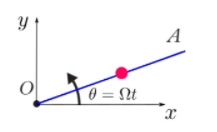
\includegraphics{1.PNG}
    \end{figure}
    
    \textbf{Sol:}
    
    Dado que la caida es sin rozamiento, se tiene que
    
    \begin{equation*}
        x = r \cos{(\Omega t)}
    \end{equation*}
    
    \begin{equation*}
        y = r \sin{(\Omega t)}
    \end{equation*}
    
    donde
    
    \begin{equation*}
        \dot{x}^2 = r^2 \sin^2{(\Omega t)} \Omega^2 + \dot{r^2} \cos^2{(\Omega t)}
    \end{equation*}
    
    \begin{equation*}
        \dot{y}^2 = r^2 \cos^2{(\Omega t)} \Omega^2  + \dot{r}^2 \sin^2{((\Omega t))}
    \end{equation*}
    
    y así el Lagrangiano es
    
    \begin{equation*}
        L = \frac{1}{2} m (\dot{x}^2 + \dot{y}^2) + mg ( r \sin{(\Omega t)})
    \end{equation*}
    
    \begin{equation*}
        = \frac{1}{2} m (\dot{r}^2 + r^2 \Omega^2) + mg ( r \sin{(\Omega t)})
    \end{equation*}
    
    \begin{equation*}
        \frac{\partial L}{ \partial r} =  m r \Omega^2  + mg \sin{(\Omega t)}  
    \end{equation*}
    
    \begin{equation*}
        \frac{\partial L}{ \partial \dot{r}} = m \dot{r}  
    \end{equation*}
    
    entonces
    
    \begin{equation*}
        \frac{d}{dt} \left(\frac{\partial L}{\partial \dot{r}}\right) - \frac{\partial L}{\partial r} = 0
    \end{equation*}
    
    \begin{equation*}
        m \ddot{r} -  m r \Omega^2  - mg \sin{(\Omega t)} = 0
    \end{equation*}
    
    
    
%%%4%%%
    
    
    
    \item Una varilla de longitud $l$, masa $m$ y densidad lineal uniforme, cuelga de un pivote sin fricción que está a una distancia $d$ de uno de sus extremos (vea la figura). La varilla es un tipo de péndulo físico sobre el que actúa la gravedad. a) Encuentre la energía cinética $T$ y la energía potencial en términos de la variable generalizada $\theta$ y su respectiva velocidad $\dot{\theta}$. b) Escribe la lagrangiana y las ecuaciones de movimiento. c) ¿Cual es el periodo de las oscilaciones si estas son pequeñas? ($\theta << 1$)
    
    \begin{figure}[h!]
        \centering
        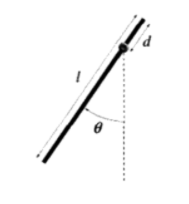
\includegraphics{2.PNG}
    \end{figure}
    
    \textbf{Sol:}
    
    La energía cinética de este problema está dada por
    
    \begin{equation*}
        T =\frac{1}{2} I \omega^2= \frac{1}{6} m (l-d)^2 \dot{\theta}^2
    \end{equation*}
    
    y con energía potencial
    
    \begin{equation*}
        U = mgh = mg (\frac{(l-d)}{2}\cos{\theta})
    \end{equation*}
    
    enotnces su lagrangiana es
    
    \begin{equation*}
        L = \frac{1}{6} m (l-d)^2 \dot{\theta}^2 - mg (\frac{(l-d)}{2}\cos{\theta})
    \end{equation*}
    
    y bien
    
    \begin{equation*}
        \frac{d}{dt} \left(\frac{\partial L}{\partial \dot{\theta}}\right) - \frac{\partial L}{\partial \theta} = 0
    \end{equation*}
    
    \begin{equation*}
        \frac{d}{dt} \left( \frac{1}{3}m (l-d)^2 \dot{\theta}\right) - mg \frac{l-d}{2}\sin{\theta} = 0
    \end{equation*}
    
    \begin{equation*}
        \frac{1}{3}m (l-d)^2 \ddot{\theta} - mg \frac{l-d}{2}\sin{\theta} = 0
    \end{equation*}
    
    si $\theta << 1$, entonces el periodo de oscilación se puede aproximar como
    
    \begin{equation*}
        2\pi \sqrt{\frac{(l-d)}{2g}} 
    \end{equation*}
    
    donde $(l-d)/2$ es el centro de masa del péndulo
    
    
    
    
%%%5%%%
    
    
    
    \item Una partícula se mueve en el plano bajo la acción de una fuerza cuya magnitud es
    
    \begin{equation*}
        F = \frac{1}{r^2} \left(1 - \frac{\dot{r}^2 - 2 r \ddot{r}}{c^2}\right)
    \end{equation*}
    
    siendo $r$ la distancia al centro de fuerzas. a) Analizar si el sistema es conservativo y hallar un potencial dependiente de $\ddot{r}$. b) Analizar si el sistema admite una formulación lagrangiana.
    
    \textbf{Sol:}
    
    F es una cantidad conservada si
    
    \begin{equation*}
        \frac{d F}{dt} = \frac{\partial F}{\partial r} \dot{r} + \frac{\partial F}{ \partial \dot{r}} \ddot{r} +\cancel{ \frac{\partial F}{\partial t} }= 0
    \end{equation*}
    
    entonces
    
    \begin{equation*}
        \frac{d F}{dt} = \left(-\frac{2}{r^3} \left(1 - \frac{\dot{r}^2 - 2r \ddot{r}}{c^2}\right) + \frac{1}{r^2} \frac{2\ddot{r}}{c^2}\right) \dot{r} - \frac{2 \dot{r}}{r^2 c^2} \ddot{r}
    \end{equation*}
    
    \begin{equation*}
        = \left(-\frac{2}{r^3} \left(1 - \frac{\dot{r}^2 - 2r \ddot{r}}{c^2}\right) + \cancel{\frac{2\ddot{r}}{c^2r^2}}\right) \dot{r} -\cancel{ \frac{2 \dot{r}}{r^2 c^2}} \ddot{r} = - \frac{2}{r} F
    \end{equation*}
    
    lo que creo que no se anula por lo que no debe ser conservativo, para obtener el potencial, recordemos que
    
    \begin{equation*}
        F= - \frac{\partial U}{\partial r} + \frac{d}{dt} \left(\frac{\partial U}{\partial \dot{r}}\right)
    \end{equation*}
    
    se tiene
    
    \begin{equation*}
        F =  \frac{1}{r^2} - \frac{\dot{r}^2}{c^2 r^2 } + \frac{2\ddot{r}^2}{c^2 r} +\left(\frac{\dot{r}^2}{c^2 r^2} - \frac{\dot{r}^2}{c^2 r^2}\right)
    \end{equation*}
    
    \begin{equation*}
        = -\left(-\frac{1}{r^2} \left( 1 + \frac{\dot{r}^2}{c^2}\right) \right) - \frac{2 \dot{r}}{c^2 r^2} \dot{r}+ \frac{2 \ddot{r}}{c^2 r} 
    \end{equation*}
    
    \begin{equation*}
        = - \frac{\partial}{\partial r} \left(\frac{1}{r} \left(1+\frac{\dot{r}^2}{c^2}\right)\right) + \frac{d}{dt} \left(\frac{1}{r} \frac{2 \dot{r}}{c^2}\right)
    \end{equation*}
    
    \begin{equation*}
        = - \frac{\partial}{\partial r} \left(\frac{1}{r} \left(1+\frac{\dot{r}^2}{c^2}\right)\right) + \frac{d}{dt} \left(\frac{\partial }{\partial \dot{r}}\left(\frac{1}{r} \left(1+\frac{\dot{r}^2}{c^2}\right)\right)\right)
    \end{equation*}
    
    \begin{equation*}
        \therefore \hspace{1cm} U = \frac{1}{r} \left(1+\frac{\dot{r}^2}{c^2}\right)
    \end{equation*}
    
    ahora que tenemos el potencial solo falta la energía cinetica para completar la lagrangiana, y como $\dot{r}^2 = \dot{r}^2 + \dot{r}^2 \dot{\theta}^2$ en coordenadas polares
    
    \begin{equation*}
        L = \frac{1}{2} m (\dot{r}^2 + \dot{r}^2 \dot{\theta}^2) - \frac{1}{r} \left(1+\frac{\dot{r}^2}{c^2}\right)
    \end{equation*}
    
    
    
    
%%%6%%%
    
    
    
    \item La lagrangiana de una partícula de carga $e$ en presencia de un campo eléctrico $\mathbf{E}$ y un campo magnético $\mathbf{B}$ es de la forma
    
    \begin{equation*}
         L = \frac{1}{2} m \dot{\mathbf{r}}^2 - e(\phi - \dot{\mathbf{r}} \cdot \mathbf{A})
    \end{equation*}
    
    donde $\phi(\mathbf{r}, t)$ es el potencial escalar y $\mathbf{A}(\mathbf{r},t)$ es el potencial vectorial, tales que
    
    \begin{equation*}
        \mathbf{E} = - \nabla \phi - \frac{\partial \mathbf{A}}{\partial t} \hspace{2cm} \mathbf{B} = \nabla \times \mathbf{A}
    \end{equation*}
    
    \begin{enumerate}
        \item Obtenga las ecuaciones de Lagrange
        
        \textbf{Sol:}
        
        Sustituyendo en
        
        \begin{equation*}
            \frac{d}{dt} \left(\frac{\partial  L}{\partial \dot{x_i}}\right) - \frac{\partial L}{\partial x_i} = 0
        \end{equation*}
        
        \begin{equation*}
            \frac{d}{dt} \left(m \dot{x}_i +e A_{x_i}\right) + e \frac{\partial \phi}{\partial x_i} - e \frac{\partial \mathbf{A}}{\partial x_i} = 0
        \end{equation*}
        
        \begin{equation*}
            e \frac{\partial A_{x_i}}{\partial x_i} \dot{x}_i + m \ddot{x}_i +   e \frac{\partial \phi}{\partial x_{i}} - e \frac{\partial \mathbf{A}}{\partial x_i} = 0
        \end{equation*}
        
       
        
        
        
        \item Demuestre que estas corresponden con la ley de fuerza de Lorentz
    
    
        
        \begin{equation*}
            m \ddot{\mathbf{r}} = e(\mathbf{E}+ \dot{\mathbf{r}} \times \mathbf{B})
        \end{equation*}
    \end{enumerate}
    
    \textbf{Sol:}
    
    Dado $L$, se puede ver que $U = e(\phi - \mathbf{\dot{r}} \cdot \mathbf{A})$,entonces como
    
    \begin{equation*}
        Q_i = - \frac{\partial U}{\partial q_i} + \frac{d}{dt} \frac{\partial U}{\partial \dot{q}_i}
    \end{equation*}
    
    se tiene que
    
    \begin{equation*}
        F_{x_i} = e\left[-\frac{\partial}{\partial x_i} \left(\phi - \dot{r} \cdot \mathbf{A}\right) + \frac{d}{dt} \frac{\partial}{\partial \dot{x}_i} \left(\phi - \dot{r} \cdot \mathbf{A}\right) \right]
    \end{equation*}
    
    \begin{equation*}
        = e\left[-\frac{\partial \phi}{\partial x_i}  +\frac{\partial}{\partial x_{i}}\left( \dot{r} \cdot \mathbf{A}\right) + \frac{d}{dt} \left( A_{x_i}\right)\right]
    \end{equation*}
        
        
    ahora como
    
    \begin{equation*}
        (\dot{r} \times \nabla \times \mathbf{A})_{x_i} = v_{x_j} \left(\frac{\partial A_{x_j}}{\partial x_i} - \frac{\partial A_{X_i}}{\partial x_j}\right) - v_{x_k} \left( \frac{\partial A_{x_i}}{\partial x_k} - \frac{\partial A_{x_k}}{\partial x_i}\right)
    \end{equation*}
    
    y
    
    \begin{equation*}
        \frac{d A_{x_i}}{d t} = \frac{\partial A_{x_i}}{\partial t} + \frac{\partial A_{x_i}}{\partial x_i} \dot{x}_i + \frac{\partial A_{x_i}}{\partial x_j} \dot{x}_j  + \frac{\partial A_{x_i}}{\partial x_k} \dot{x}_k
    \end{equation*}
    
    entonces
    
    \begin{equation*}
        (\dot{r} \times \nabla \times \mathbf{A})_{x_i} = \frac{\partial}{\partial x_i} (\dot{r} \cdot \mathbf{A}) - \frac{d A_{x_i}}{d t} + \frac{\partial A_{x_i}}{\partial x_i}
    \end{equation*}
    
    que sustituyendo
    
    \begin{equation*}
        F_{x_i} = e \left[-\frac{\partial \phi}{\partial x_i} - \frac{\partial A_{x_i}}{\partial t} + (\dot{r} \times \nabla \times \mathbf{A})_{x_i} \right]
    \end{equation*}
    
    \begin{equation*}
        F_{x_i} = e \left[-\frac{\partial \phi}{\partial x_i} - \frac{\partial A_{x_i}}{\partial t} + (\dot{r} \times \mathbf{B})_{x_i} \right]
    \end{equation*}
    
    o bien
    
    \begin{equation*}
         F = e \left[-\nabla \phi - \frac{\partial \mathbf{A}}{\partial t} + \dot{r} \times \mathbf{B} \right]
    \end{equation*}
    
    \begin{equation*}
       = e \left[\mathbf{E} + \dot{r} \times \mathbf{B} \right]
    \end{equation*}
    
    
    
    
%%%7%%%
        
        
        
        \item Calcular la curva geodésica que une a dos puntos sobre un cono. Para ello recordar que la ecuación de un cono en coordenadas cilíndricas ($\rho, \phi, z$) es:
        
        \begin{equation*}
            \rho = \lambda z \hspace{1cm} \lambda \in R
        \end{equation*}
        
        \textbf{Sol:}
        
        Para coordenadas cilíndricas, el diferencial de linea es
        
        \begin{equation*}
            ds^2 = d\rho^2 + \rho^2 d\phi^2 + dz^2 = d\rho^2 + \rho^2 d\phi^2 + \frac{d\rho^2}{\lambda^2}
        \end{equation*}
        
        \begin{equation*}
            = \frac{1 + \lambda^2}{\lambda^2} d \rho^2 + \rho^2 d\phi^2
        \end{equation*}
        
        ahora sustituyendo esto en la expresión para la longitud de arco
        
        \begin{equation*}
            \int ds = \int \sqrt{\frac{1 + \lambda^2}{\lambda^2} d \rho^2 + \rho^2 d\phi^2} = \int d\rho \sqrt{\frac{1 + \lambda^2}{\lambda^2} + \rho^2 \dot{\phi}^2}
        \end{equation*}
        
        con \begin{equation*}
            F(\rho, \dot{\phi}) =\sqrt{ \frac{1 + \lambda^2}{\lambda^2} + \rho^2 \dot{\phi}^2}
        \end{equation*}
        
        que usando las ecuaciones de Euler-Lagrange
        
        \begin{equation*}
            \frac{d}{d\rho} \left(\frac{\partial F}{\partial \dot{\phi}}\right) - \cancel{\frac{\partial F}{\partial \phi}} = 0
        \end{equation*}
        
        \begin{equation*}
            \frac{d}{d\rho} \left( \frac{\rho^2 \dot{\phi}}{\sqrt{ \frac{1 + \lambda^2}{\lambda^2} + \rho^2 \dot{\phi}^2}} \right) = 0
        \end{equation*}
        
        o bien
        
        \begin{equation*}
            \frac{\rho^2 \dot{\phi}}{\sqrt{ \frac{1 + \lambda^2}{\lambda^2} + \rho^2 \dot{\phi}^2}} = c  \hspace{5cm} c = cte
        \end{equation*}
        
        y desarrollando
        
        \begin{equation*}
            \rho^4 \dot{\phi}^2 = c^2\left( \frac{1 + \lambda^2}{\lambda^2} + \rho^2 \dot{\phi}^2\right)
        \end{equation*}
        
        \begin{equation*}
            \dot{\phi}^2(\rho^4 -c^2 \rho^2) = c^2 \frac{1 + \lambda^2}{\lambda^2} 
        \end{equation*}
        
        
        \begin{equation*}
            \dot{{\phi}} = \frac{c \sqrt{\frac{1 + \lambda^2}{\lambda^2}} }{\rho\sqrt{\rho^2 -c^2}}
        \end{equation*}
        
        \begin{equation*}
            \int d\phi =c \sqrt{\frac{1 + \lambda^2}{\lambda^2}} \int  \frac{d\rho }{\rho\sqrt{\rho^2 -c^2}}
        \end{equation*}
        
        Sea $\rho = c \sec{\theta}$ y $d \rho = c \sec{\theta} \tan{\theta} d \theta$, también como $\sec^2{\theta} - 1 = \tan^2{\theta}$
        
        \begin{equation*}
            \int d\phi = \sqrt{\frac{1 + \lambda^2}{\lambda^2}} \int  \frac{\cancel{c^2 \sec{\theta} \tan{\theta}} d\theta}{\cancel{c^2 \sec{\theta}\tan{\theta}
            }}
        \end{equation*}
        
        \begin{equation*}
            \phi + k = \sqrt{\frac{1 + \lambda^2}{\lambda^2}} \theta=   \sqrt{\frac{1 + \lambda^2}{\lambda^2}} \cos^{-1}{\frac{c}{\rho}}
        \end{equation*}
        
        \begin{equation*}
            c = \rho \cos{\frac{\phi + k
            }{  \sqrt{\frac{1 + \lambda^2}{\lambda^2}}}}
        \end{equation*}
        
        
        
        
        
%%%8%%%
        
        
        
        \item Calcular la curva que genera una cuerda de densidad lineal uniforme $\lambda$. La cuerda está sujeta a la gravedad y sus extremos son fijos.
        
        \textbf{Sol:}
        
        La longitud de arco en cartesianas es
        
        \begin{equation*}
            L = \int ds = \int dx \sqrt{1+ \dot{y}^2}
        \end{equation*}
        
        pero como la cuerda está estática, se tiene que su energía potencial debida al campo gravitatorio es constante y además
        
        \begin{equation*}
            U =mgh = \lambda L g y =  \int dx \lambda g y \sqrt{1 + \dot{y}^2}
        \end{equation*}
        
        y usando las ecuaciones de Lagrange en la forma de Beltromi con $F= \lambda g y \sqrt{1+ \dot{y}^2}$
        
        \begin{equation*}
            \frac{d}{d x}\left( \dot{y}\frac{\partial F}{\partial \dot{y}}-F\right) = 0
        \end{equation*}
        
        \begin{equation*}
            \frac{d}{d x}\left(\frac{\lambda g y \dot{y}^2}{\sqrt{1 + \dot{y}^2}} -  \lambda g  y \sqrt{1 + \dot{y}^2} \right) = 0
        \end{equation*}
        
        o bien
        
        \begin{equation*}
             \frac{\lambda g y \dot{y}^2}{\sqrt{1 + \dot{y}^2}} -  \lambda g  y \sqrt{1 + \dot{y}^2} = c
        \end{equation*}
        
        \begin{equation*}
            \lambda g y\left(\frac{\dot{y}^2}{\sqrt{1 + \dot{y}^2}} -  \sqrt{1 + \dot{y}^2}\right) = c
        \end{equation*}
        
         \begin{equation*}
             \lambda g y \left(\frac{-1}{\sqrt{1+ \dot{y}^2}} \right) = c
         \end{equation*}
         
         \begin{equation*}
             \dot{y}^2 = \frac{\lambda^2 g^2 y^2}{c^2} - 1
         \end{equation*}
         
         Sea $u = \lambda g y /c$ y $du = \lambda g/c dy$
         
         \begin{equation*}
              \int \frac{du}{\sqrt{u^2 - 1}} = \int \frac{\lambda g}{c} dx
         \end{equation*}
         
         Sea $u = \cosh{w}$, $du = \sinh{w} dw$
         
         \begin{equation*}
             \int dw = \frac{\lambda g}{c} x + c
         \end{equation*}
         
         \begin{equation*}
             w = \cosh^{-1}{u} = \frac{\lambda g}{c} x + c
         \end{equation*}
         
         \begin{equation*}
             y = \frac{c}{\lambda g} \cosh{(\frac{\lambda g}{c} x + c)}
         \end{equation*}
        
        
        
        
        
%%%9%%%
        
        
        
        \item Una partícula de masa $m$ se mueve en el plano $xy$ y está sometida a un potencial de la forma $V(x-2y)$
        
        \begin{enumerate}
            \item Demuestre que la lagrangiana es invariante ante un grupo de traslaciones oblicuoas (Hint: Si $x$ es incrementada en cantidad arbitraria $s$, ¿qué cantidad debe incrementarse $y$ para que el potencial no cambie?)
            
            \textbf{Sol:}
            
            Para ver que la lagrangiana es invariante respecto a la transformación $(x,s) \rightarrow (x+s,y+\frac{1}{2}s)$, se tiene que mostrar
            
            \begin{equation*}
                L(x,y,\dot{x,\dot{y}}) = L(x+s,y+\frac{1}{2}s, \dot{(x+s)},\dot{(y+\frac{1}{2}s)})
            \end{equation*}
            
            entonces
            
            \begin{equation*}
                L(x+s,y+\frac{1}{2}s, \dot{(x+s)},\dot{(y+\frac{1}{2}s)}) =\frac{1}{2}m (\dot{(x+s)}^2 + \dot{y+\frac{1}{2}s}^2) - V(x+s - 2(y + \frac{1}{2}s))
            \end{equation*}
            
            \begin{equation*}
                =\frac{1}{2} m (\dot{x}^2 + \dot{y}^2)  - V(x+\cancel{s}-2y\cancel{-s}) = L(x,y,\dot{x},\dot{y})
            \end{equation*}
            
            por lo tanto $L$ es invariante ante transformaciones oblicuas
            
            
            \item Con ayuda del teorema de Noether muestre que la cantidad $\dot{x} + \frac{1}{2} \dot{y}$ es una constante de movimiento
            
            \textbf{Sol:}
            
            Por el teorema de Noether, y por el ejemplo 1 de la presentación de teoremas de conservación, se tiene
            
            \begin{equation*}
                \frac{\partial L}{\partial \dot{x}} = m\dot{x}= p_x
            \end{equation*}
            
            \begin{equation*}
                \frac{\partial L}{\partial \dot{y}} = m\dot{y} = p_y
            \end{equation*}
            
            son cantidades conservadas, y entonces
            
            \begin{equation*}
                m\ddot{x} = 0 \hspace{1cm} \rightarrow \hspace{1cm} \ddot{x} = 0
            \end{equation*}
            
            \begin{equation*}
                m\ddot{y} = 0 \hspace{1cm} \rightarrow \hspace{1cm} \frac{1}{2} \ddot{y} = 0
            \end{equation*}
            
            \begin{equation*}
                \ddot{x} + \frac{1}{2} \ddot{y} = 0
            \end{equation*}
            
            pero esto es igual a 
            
            \begin{equation*}
                \frac{\partial F}{\partial \dot{x}} \ddot{x} + \frac{\partial F}{\partial \dot{y}} \ddot{y} + \frac{\partial F}{\partial t} = 0
            \end{equation*}
            
            con $F= \dot{x} + \frac{1}{2} \dot{y}$ por lo que $F$ es una cantidad conservada
            
            
            
        \end{enumerate}
        
        
        
%%%10%%%
        
        
        \item En ciertas situaciones, particularmente en sistema unidimensionales, se pueden incorporar los efectos del rozamiento sin introducir la función de disipación. A título de ejemplo,
        
        a) hallar las ecuaciones del movimiento para la lagrangiana
        
        \begin{equation*}
            L(x,\dot{x}, t) = \frac{1}{2} e^{\alpha t} (\dot{x}^2 - \omega^2 x^2)
        \end{equation*}
        
        \textbf{Sol:}
        
        Como $L(x,\dot{x},t)$,
        
        \begin{equation*}
            \frac{d}{dt}\left(\frac{\partial L}{\partial \dot{x}}\right) - \frac{\partial L}{\partial x} = 0
        \end{equation*}
        
        \begin{equation*}
            \frac{d}{dt}\left(e^{\alpha t} \dot{x}\right) + e^{\alpha t} \omega^2 x = 0
        \end{equation*}
        
        \begin{equation*}
            e^{\alpha t} \ddot{x} + \alpha e^{\alpha t} \dot{x} + e^{\alpha t} \omega^2 x = 0
        \end{equation*}
        
        \begin{equation*}
            e^{\alpha t}( \ddot{x} + \alpha \dot{x} +  \omega^2 x)= 0
        \end{equation*}
        
        y como $e^{\alpha} t > 0$
        
        \begin{equation*}
            \ddot{x} + \alpha \dot{x} +  \omega^2 x= 0
        \end{equation*}
        
        
        b) ¿Existen constantes de movimiento?
        
        \textbf{Sol:}
        
        La lagrangiana depende del tiempo así que su hamiltoniano no debe ser una constante de movimiento, lo mismo para la lagrangiana, energía cinética, potencial, momento conjugado y ya no se me ocurre otra más
        
        %\newpage
        
        
        
%%%11%%%
        
        
        
        \item Una cuenta de masa $m$  está obligada a moverse sin fricción sobre un arco de radio $R$ que gira alrededor de la vertical con velocidad angular constante $\Omega$ (vea la figura). a) Obtener las ecuaciones de Lagrange suponiendo que las fuerzas exteriores son únicamente las debidas a la gravedad. b) Encuentre el hamiltoniano $H$. ¿Es $H$ una constante de movimiento? ¿Es la energía ($T+V$) constante? c) Demostrar que si $\Omega$ es mayor que un cierto valor crítico $\Omega_0$, puede haber una solución en la cual la partícula permanece fija en el arco en un punto que no es el más bajo, pero que si $\Omega < \Omega_0$, el único punto estacionario para la partícula es el más bajo del arco ¿Cuál es el valor de $\Omega_0$?
        
        \begin{figure}[h!]
            \centering
            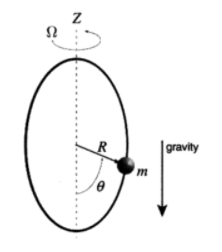
\includegraphics{3.PNG}
        \end{figure}
        
        \textbf{Sol:}
        
        Dadas las condiciones dadas, el problema se describe como
        
        \begin{equation*}
            x = a \sin{\theta} \cos{\Omega t}
        \end{equation*}
        
        \begin{equation*}
            y = a \sin{\theta} \sin{\Omega t}
        \end{equation*}
        
        \begin{equation*}
            z = a \cos{\theta}
        \end{equation*}
        
        entonces la energía cinética es
        
        \begin{equation*}
            T = \frac{1}{2} m (\dot{x}^2 + \dot{y}^2 + \dot{z}^2) = \frac{m}{2} [(a\cos{\theta}\cos{\Omega t} \dot{\theta} - a \Omega \sin{\theta}\sin{\Omega t} )^2 + (a \cos{\theta}\sin{\Omega t} \dot{\theta} + a \Omega \sin{\theta} \cos{\Omega t})^2
        \end{equation*}
        
        \begin{equation*}
             + (a\sin{\theta}\dot{\theta})^2]
        \end{equation*}
        
        \begin{equation*}
            = \frac{ma^2}{2}[\cos^2{\theta} \dot{\theta}^2 \cancel{(\cos^2{\Omega t} + \sin^2{\Omega t})} + w^2 \sin^2{\theta} \cancel{(\cos^2{\Omega t} + \sin^2{\Omega t})}\pm \cancel{2\Omega \cos{\theta}\sin{\theta}\cos{\Omega t} \dot{\theta}} + \sin^2{\theta}\dot{\theta}^2
        \end{equation*}
        
        \begin{equation*}
            = \frac{ma^2}{2}\cancel{(\dot{\theta}^2 (\cos^2{\theta} + \sin^2{\theta})} + \Omega^2 \sin^2{\theta})
        \end{equation*}
        
        entonces la lagrangiana es
        
        \begin{equation*}
            L = \frac{ma^2}{2}(\dot{\theta}^2 + \Omega^2 \sin^2{\theta})   + mga \cos{\theta}
        \end{equation*}
        
        y así la ec. de mivimiento es
        
        \begin{equation*}
            \frac{d}{dt}\left(\frac{\partial L}{\partial \dot{\theta}}\right) - \frac{\partial L}{\partial \theta} = 0
        \end{equation*}
        
        \begin{equation*}
            \frac{d}{dt}\left(\frac{\partial L}{\partial \dot{\theta}}\right) - ma^2\Omega^2 \cos{\theta} \sin{\theta} + mga \sin{\theta} = 0
        \end{equation*}
        
        \begin{equation*}
            \frac{d}{dt}\left(ma^2 \dot{\theta}\right) - ma\Omega^2 \cos{\theta} \sin{\theta}  + mga \sin{\theta} = 0
        \end{equation*}
        
        \begin{equation*}
            ma^2 (\ddot{\theta} -  \Omega^2 \cos{\theta} \sin{\theta} + \frac{g}{a} \sin{\theta}) = 0
        \end{equation*}
        
        \begin{equation*}
            \ddot{\theta} -  \Omega^2 \cos{\theta} \sin{\theta} + \frac{g}{a} \sin{\theta} = 0
        \end{equation*}
        
        El hamiltoniano es
        
        \begin{equation*}
            H = \frac{\partial L}{\partial \dot{\theta}} \dot{\theta} - L
        \end{equation*}
        
        \begin{equation*}
             = ma^2 \dot{\theta} \dot{\theta} - \frac{ma^2}{2}(\dot{\theta}^2 + \Omega^2 \sin^2{\theta})   - mga \cos{\theta}
        \end{equation*}
        
        \begin{equation*}
            = \frac{ma^2}{2} \left( \dot{\theta}^2 - \Omega^2 \sin^2{\theta} - \frac{2g}{a}\cos{\theta} \right)
        \end{equation*}
        
        y por el ejemplo 2 de la presentación de teoremas de conservación sabemos que como $L$ no depende explícitamente de $t$, entonces $H$ es una cantidad conservada.
        
        
        Ahora para que la masa se quede estática sobre el arco, se bebe tener que $\theta = \theta_0$ o bien $\ddot{\theta} = 0$ que sustituyendo
        
        \begin{equation*}
             0 = \Omega^2 \cos{\theta_0}\sin{\theta_0} - \frac{g}{a} \sin{\theta_0} = \sin{\theta_0} (\Omega^2 \cos{\theta_0} - \frac{g}{a})
        \end{equation*}
        
        entonces $\sin{\theta_0} = 0$ o $\Omega^2 \cos{\theta_0} = \frac{g}{a}$lo que se cumple para$\theta_0  = n\pi$  que es cuando la masa está en el punto más bajo o más alto y cuando $0<\frac{g}{\Omega^2 a} \leq 1$ ya que $g,a,\Omega$ son valores positivos y $\cos{\theta}$ está restringido, entonces la masa se matiene estatica para dos casos $\theta = n\pi$ y cuando $\sqrt{\frac{g}{a}} < \Omega$
        
        
        
%%%12%%%
        
        
        
        \item Una partícula de masa $m$ desliza sin rozamiento por una cuña de ángulo $\alpha$ y masa $M$ que puede deslizar sin rozamiento sobre una superficie lisa horizontal (vea la figura). Tratando la ligadura de la partícula sobre la cuña por el método de los multiplicadores de Lagrange, a) hallar las ecuaciones del movimiento de la partícula y la cuña. b) integra las ecuaciones suponiendo que en el instante inicial ambas estaban en reposo y la partícula se encontraba a una altura $h$. c) ¿Cuáles son las constantes de movimiento del sistema?
        
        \begin{figure}[h!]
            \centering
            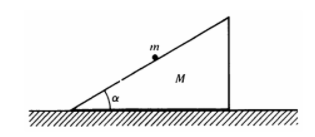
\includegraphics{4.PNG}
        \end{figure}
        
        \textbf{Sol:}
        
        Pongamos el origen en la punta inferior de la cuña al tiempo $t = 0$, entonces sea  $x'$ la distancia recorrida por la cuña desde el origen a la punta inferior al tiempo $t$ y sea $l$ la distancia de la punta inferir a la masa $m$ en el tiempo $t$, así este sistema se puede describir como
        
        \begin{equation*}
            x = x' + l\cos{\alpha}
        \end{equation*}
        
        \begin{equation*}
            y = l\sin{\alpha}
        \end{equation*}
        
        la lagrangiana del sistema es
        
        \begin{equation*}
            L = \frac{1}{2}m (\dot{x}^2 + \dot{y}^2) + \frac{1}{2}M \dot{x'}^2 + mgy
        \end{equation*}
        
        y para las ligaduras del sistema usemos que $(x- x')\sin{\theta} = l \cos{\theta}$ y $y \cos{\alpha} = l \sin{\alpha}\cos{\alpha}$
        
        \begin{equation*}
            (x-x')\sin{\alpha} - y \cos{\alpha} = 0
        \end{equation*}
        
        entonces sustituyendo
        
        \begin{equation*}
            \frac{d}{dt}\left(\frac{\partial L}{\partial \dot{x}}\right) - \frac{\partial L}{\partial x} = \lambda \frac{\partial f}{\partial x}
        \end{equation*}
        
        \begin{equation*}
            \frac{d}{dt}\left(m\dot{x}\right) - \cancel{\frac{\partial L}{\partial x}
            }= \lambda \sin{\theta}
        \end{equation*}
        
        \begin{equation}
            m\ddot{x} = \lambda \sin{\theta}
        \end{equation}
        
        \begin{equation*}
            \frac{d}{dt}\left(\frac{\partial L}{\partial \dot{x'}}\right) - \frac{\partial L}{\partial x'} = \lambda \frac{\partial f}{\partial x'}
        \end{equation*}
        
        \begin{equation*}
            \frac{d}{dt}\left(M\dot{x}'\right) - \cancel{\frac{\partial L}{\partial x'}} =- \lambda \sin{\alpha}
        \end{equation*}
        
        \begin{equation}
            M\ddot{x}' = - \lambda \sin{\alpha} 
        \end{equation}
        
        \begin{equation*}
            \frac{d}{dt}\left(\frac{\partial L}{\partial \dot{y}}\right) - \frac{\partial L}{\partial y} = \lambda \frac{\partial f}{\partial y}
        \end{equation*}
        
        \begin{equation*}
            \frac{d}{dt}\left(m\dot{y}\right) - mg =  - \lambda  \cos{\alpha}
        \end{equation*}
        
        \begin{equation}
            m\ddot{y} - mg =  - \lambda  \cos{\alpha}
        \end{equation}
        
        para (1)
        
        \begin{equation*}
            \int m d\dot{x} = \int \lambda \sin{\alpha} dt
        \end{equation*}
        
        \begin{equation*}
            \int m dx = \int\lambda \sin{\alpha} t dt
        \end{equation*}
        
        \begin{equation*}
            m x = \lambda \frac{t^2}{2} \sin{\alpha} + c
        \end{equation*}
        
        para (2)
        
        \begin{equation*}
            m x' = -\lambda \frac{t^2}{2} \sin{\alpha} + c'
        \end{equation*}
        
        para (3)
        
        \begin{equation*}
            m y = (mg-\lambda \cos{\alpha})\frac{t^2}{2} + c''
        \end{equation*}
        
        y como $y(0) = h$, $x'(0) = 0$ y $x(0) = x_0$, entonces $c = mx_0$, $c' = 0$ y $c'' = mh$
        
        
        
        
        
        como la lagrangiana no depende explícitamente de $x$, por el ejemplo 1 de la presentación de teoremas de conservación, se tiene que $\frac{\partial L}{\partial \dot{x}}$ es una cantidad conservada
        
        \begin{equation*}
            H = \frac{\partial L}{\partial \dot{x}} \dot{x} + \frac{\partial L}{\partial \dot{y}}  \dot{y} + \frac{\partial L}{\partial \dot{x}'} \dot{x}' - L
        \end{equation*}
        
        \begin{equation*}
            = \cancel{m \dot{x}^2 + m  \dot{y}^2 }+ \cancel{M \dot{x}'^2}  - \cancel{\frac{1}{2}m (\dot{x}^2 + \dot{y}^2) }- \cancel{\frac{1}{2}M \dot{x'}^2} - mgy
        \end{equation*}
        
        \begin{equation*}
            = \frac{1}{2}m (\dot{x}^2 + \dot{y}^2) + \frac{1}{2} M \dot{x}'^2 - mgy
        \end{equation*}
        
        Esta cantidad se conserva ya que $L$ no depende explícitamente del tiempo  y por el ejemplo 2
        
        
        
        
        

    
\end{enumerate}

\end{document}